\documentclass[addpoints]{exam}
\usepackage{amsmath,amsthm,amssymb,url}

\usepackage{algorithm}
\usepackage{algorithmic}
\usepackage{graphicx}
\usepackage{float}
\usepackage{units}
%\usepackage{algpseudocode}

\usepackage[pdftex]{hyperref}
\usepackage{tikz}
\usepackage{pgfplots}
\usetikzlibrary{calc,3d,decorations.markings, backgrounds, positioning,intersections,shapes}

\renewcommand{\algorithmicrequire}{\textbf{Input:}}
\renewcommand{\algorithmicensure}{\textbf{Output:}}
%\algnewcommand\algorithmicparfor{\textbf{parallel for}}
%\algdef{S}[FOR]{PFOR}[1]{\algorithmicparfor\ #1\ \algorithmicdo}

\newcommand{\BigO}[1]{\mathcal{O}\left( #1\right)}
\newcommand{\ceil}[1]{\left \lceil #1 \right \rceil }
\newcommand{\floor}[1]{\left \lfloor #1 \right \rfloor }


\newtheorem{lemma}{Lemma}[section]
\newcommand{\var}{\text{Var}}
\title{CS 6230: Homework 4}
\date{Due Date: March 13, 2016}
\author{Christopher Mertin}
\begin{document}
\maketitle
%\begin{center}
%\fbox{\fbox{\parbox{5.5in}{\centering
%This assignment has \numquestions\ questions, for a total of \numpoints\
%points.
%Unless otherwise specified, complete and reasoned arguments will be
%expected for all answers. 
%}}}
%\end{center}

\qformat{Question \thequestion: \thequestiontitle\dotfill}
\pointname{}
\bonuspointname{}
\pointformat{[\bfseries\thepoints]}

\printanswers



\begin{questions}

\titledquestion{Bitonic Sorting: Multiple Input Sizes}
How would you modify the bitonic sort algorithm if the number of input keys are arbitrary. For example, assume that as input you get $n = rank$ keys per process. While you are not required to maintain the same number of keys per process for all stages of the bitonic sort, you should not explicitly balance the distribution of the sort before sorting. In other words, any load balancing must happen as part of the bitonic sort.

{\em Hint}: While merging two bitonic sequences of unequal lenths, what needs to be done to ensure that the resulting sequences are bitonic and satisfy the $low \leq high$ requirement.

\begin{solution}
A bitonic sequence is built such as a ``rise then falls'' or a ``falls than rises'' sequence. This point in the middle is known as the {\em pivot point} of the array. You can perform it on an arbitrary sequence on $p$ nodes in the following way. 

First, you would have to sort the invididual arrays on each node. Then, after sorting, you would have to compare the values on the nodes. For example, $p_{1}$ would compare its values for the pivot point of $p_{2}$, and vice-versa. 

When a swap is supposed to take place, each node has no idea how many items the other node is going to send/receive since they are uneven. Therefore, before sending and receiving, $p_{1}$ would have to tell $p_{2}$ how many elements it was going to send, and $p_{2}$ would have to tell $p_{1}$.

From here, you would have to figure out how to deal with the different number of elements. The easiest approach would be to resize the arrays to how much more memory you're going to need before initiating the send/receive between the nodes.

To achieve proper load balancing and make it more efficient, you would resize the array to be $\left[\frac{a+b}{2} \right]$ where $a$ and $b$ are the size of the elements on $p_{1}$ and $p_{2}$, respectively. Then, when you send the data you would send it to this new size such that each of the two nodes would have the same number of elements. In sorting all the data, each node would wind up having {\em roughly} the same number of elements.
\end{solution}
\ \newpage
\titledquestion{Bitonic Sort}
Implement an MPI parallel bitonic sort algorithm. You can assume that the number of input keys per process will be the same. The number of processes can be arbitrary. Write a driver routine called \verb~sort~ that takes one argument, the size of the array to be sorted (initialized to random integers). On the write-up, give pseudocode for your algorithm, and report wall clock time/core/$n$ results for $n/p = 1, 10, 100, 1000, 1M$ elements using 16 MPI tasks per node for as large a number of nodes as possible. At least try for $1,2,3,4$ nodes. Report weak and strong scaling results.

\begin{solution}
The implemented solution to this problem first performs a {\em local} bitonic sort on the data for each node, which can be seen in Algorithm~\ref{alg:bitonic_seq}. After which, it calls another funciton which sorts it via the bitonic sort algorithm between each node with Algorithm~\ref{alg:bitonic_mpi}. The pseudocode for each was taken from a source and converted into {\tt C++} code. The respective sources are labeled next to each algorithm.

The results for the timings can be found in Table~\ref{table:times}. To obtain these timings, each task was run 10 times and the average timings were taken. The strong scaling results can be seen in Figure~\ref{fig:strong_scaling} while the results for the weak scaling can be found in Figure~\ref{fig:weak_scaling}.


\begin{algorithm}[H]
\caption{$BitonicSort(low,high,up,A)$ \cite{bitonic}}
\begin{algorithmic}
\REQUIRE{$low$est variable to sort, $high$est variable to sort, $A\in \mathbb{R}^{n\times 1}$, boolean $up$ for ascending order}
\ENSURE{$A\in \mathbb{R}^{n\times 1}$ sorted}
\IF{$high > 1$}
\STATE{$midPoint\leftarrow high/2$}
\STATE{$BitonicSort(low, midPoint, A, \text{\bf not }up)$}
\STATE{$BitonicSort(low + midPoint, high-midPoint, A, up)$}
\STATE{$BitonicMerge(low, high, A, up)$ [see Algorithm~\ref{alg:bitonic_Merge}]}
\ENDIF
\end{algorithmic}
\label{alg:bitonic_seq}
\end{algorithm}

\begin{algorithm}[H]
\caption{$BitonicMerge(low,high,up,A)$ \cite{bitonic}}
\begin{algorithmic}
\REQUIRE{$low$est variable to sort, $high$est variable to sort, $A\in \mathbb{R}^{n\times 1}$, boolean $up$ for ascending order}
\IF{$high > 1$}
\STATE{$m\leftarrow $Greatest Powrer of 2 less than $high$}
\FOR{$i = low$ \TO $low + high - m - 1$}
    \IF{$(A_{low} > A_{high}) = up$}
       \STATE{$swap(A_{low},A_{high})$}
    \ENDIF
\ENDFOR
\STATE{$BitonicMerge(low, m, A, up)$}
\STATE{$BitonicMerge(low + m, high - m, A, up)$}
\ENDIF
\end{algorithmic}
\label{alg:bitonic_Merge}
\end{algorithm}

\begin{algorithm}[H]
\caption{Parallel Bitonic Sorting \cite{bitonicMPI}}
\begin{algorithmic}
\REQUIRE{$A\in \mathbb{R}^{n\times 1}$ (sorted), $numNodes$, $nodeID$}
\ENSURE{$A\in \mathbb{R}^{n\times 1}$ sorted between the nodes}
\FOR{$i = 1$ \TO $\log_{2}(numNodes)$}
    \STATE{$nodeBit \leftarrow$ Most significant $(d-i)$ bits of $nodeID$}
    \FOR{$j = i-1$ \TO 0}
        \IF{($nodeBit \in \text{even}$ \AND $j^{th}$ bit of $nodeID = 0$) \OR ($nodeID \in \text{odd}$ \AND $j^{th}$ bit of $nodeID = 1$)}
           \STATE{$CompareLow(j)$}
           \COMMENT{Starts merging from the high end between nodes}
        \ELSE
           \STATE{$CompareHigh(j)$}
           \COMMENT{Starts merging from the low end between nodes}
        \ENDIF
        \STATE{$BitonicSort(A)$}
        \COMMENT{sequential}
    \ENDFOR
\ENDFOR
\end{algorithmic}
\label{alg:bitonic_mpi}
\end{algorithm}


\begin{table}[H]
\centering
\caption{Average Bitonic Sort Timings}
\begin{tabular}{ c c c c c c c c c}
\hline\hline
Nodes & $10^{0}$ & $10^{1}$ & $10^{2}$ & $10^{3}$ & $10^{4}$ & $10^{5}$ & $10^{6}$ & $10^{7}$ \\
\hline
1 & 0.0001 & 0.0003 & 0.0007 & 0.0050 & 0.0521 & 0.4597 & 3.1554 & 37.0015\\
2 & 0.0002 & 0.0005 & 0.0011 & 0.0074 & 0.0932 & 1.0341 & 4.7064 & 53.4787\\
4 & 0.0004 & 0.0007 & 0.0026 & 0.0170 & 0.1507 & 1.1991 & 6.6821 & 73.5433\\
8 & 0.0005 & 0.0022 & 0.0040 & 0.0242 & 0.1940 & 1.2787 & 8.8620 & 96.9317\\
16 & 0.0006 & 0.0032 & 0.0288 & 0.0378 & 0.2421 & 1.5918 & 10.9514 & 125.2008\\
32 & 0.0005 & 0.0037 & 0.0230 & 0.4341 & 0.3226 & 1.7681 & 14.0641 & 157.7905\\
\hline\hline
\multicolumn{9}{l}{\scriptsize $\dagger$ Each node was assigned 16 MPI Processes}\\
\multicolumn{9}{l}{\scriptsize $\ddagger$ Given values are in seconds}
\end{tabular}
\label{table:times}
\end{table}

\begin{figure}[H]
\centering
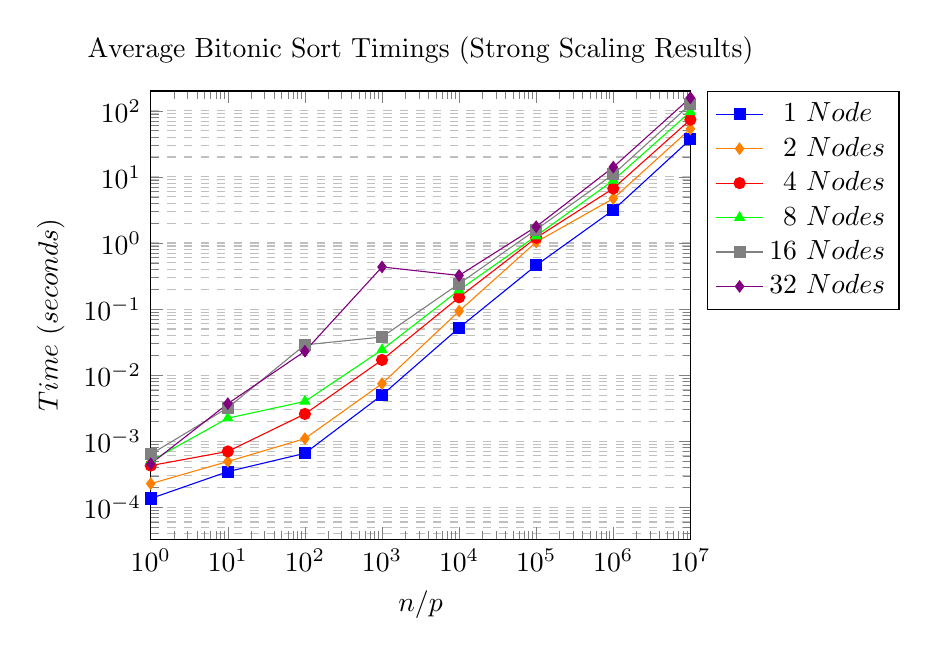
\begin{tikzpicture}
\begin{axis}[
    title={Average Bitonic Sort Timings (Strong Scaling Results)}, xlabel={$n/p$}, ylabel={$Time\ (seconds)$}, xmin=1, xmax=10000000, ymin=0, ymax=200, xmode=log,ymode=log, legend pos=outer north east,ymajorgrids=true,yminorgrids=true,grid style=dashed,]%ytick={0, .1, .2, .3, .4, .5, .6, .7, .8, .9, 1.0},]
% Nodes = 1
\addplot[color=blue, mark=square*,]
	coordinates{(1,0.00013595)(10,0.00034704)(100,0.00065694)(1000,0.00499825)(10000,0.05211904)(100000,0.45973560)(1000000,3.15541400)(10000000,37.00154000)};
% Nodes = 2
\addplot[color=orange, mark=diamond*,]
	coordinates{(1,0.00022798)(10,0.00049367)(100,0.00109620)(1000,0.00743699)(10000,0.09322842)(100000,1.03408160)(1000000,4.70643600)(10000000,53.47866000)};
% Nodes = 4
\addplot[color=red, mark=*,]
	coordinates{(1,0.00042831)(10,0.00070100)(100,0.00258849)(1000,0.01698379)(10000,0.15068580)(100000,1.19905720)(1000000,6.68207800)(10000000,73.54334000)};
% Nodes = 8
\addplot[color=green, mark=triangle*,]
	coordinates{(1,0.00050101)(10,0.00223461)(100,0.00400695)(1000,0.02415056)(10000,0.19400360)(100000,1.27865650)(1000000,8.86200700)(10000000,96.93174000)};
% Nodes = 16
\addplot[color=gray, mark=square*,]
	coordinates{(1,0.00063595)(10,0.00321116)(100,0.02879230)(1000,0.03776743)(10000,0.24205800)(100000,1.59176000)(1000000,10.95137000)(10000000,125.20080000)};
% Nodes = 32
\addplot[color=violet, mark=diamond*,]
	coordinates{(1,0.00045523)(10,0.00370514)(100,0.02300932)(1000,0.43406650)(10000,0.32263990)(100000,1.76809200)(1000000,14.06411000)(10000000,157.79050000)};
\legend{$\phantom{1}1\ Node\phantom{s}$, $\phantom{1}2\ Nodes$, $\phantom{1}4\ Nodes$, $\phantom{1}8\ Nodes$, $16\ Nodes$, $32\ Nodes$}
\end{axis}
\end{tikzpicture}
\caption{Each node was assigned 16 MPI Processes}
\label{fig:strong_scaling}
\end{figure}

\begin{figure}[H]
\centering
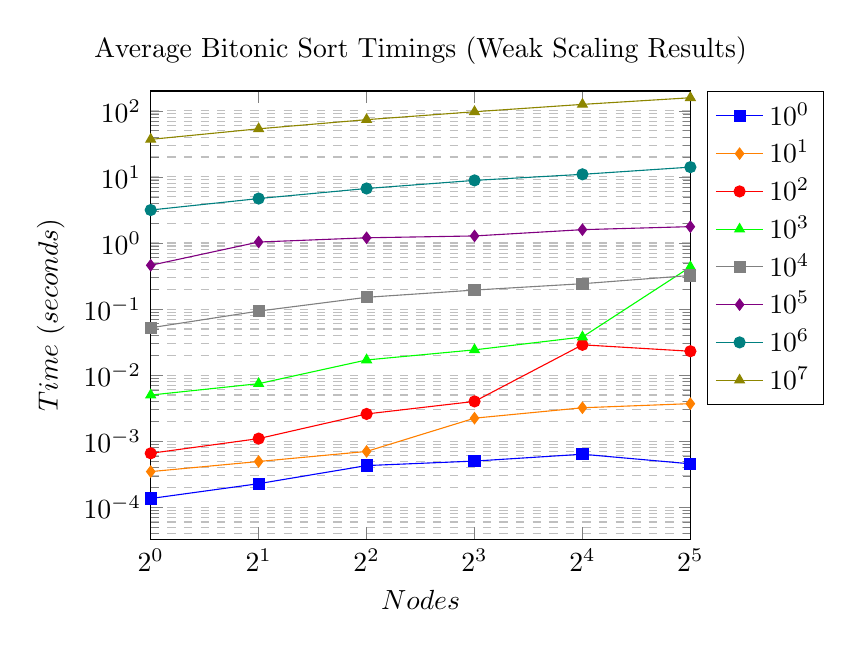
\begin{tikzpicture}
\begin{axis}[
    title={Average Bitonic Sort Timings (Weak Scaling Results)}, xlabel={$Nodes$}, ylabel={$Time\ (seconds)$}, xmin=1, xmax=32, ymin=0, ymax=200,ymode=log, xmode=log,log basis x={2}, legend pos=outer north east,ymajorgrids=true,yminorgrids=true,grid style=dashed]
% n = 1
\addplot[color=blue, mark=square*,]
	coordinates{(1, 0.00013594618)(2, 0.0002279758)(4, 0.000428305)(8, 0.0005010129)(16, 0.000635953)(32, 0.0004552337)};
% n = 10
\addplot[color=orange, mark=diamond*,]
	coordinates{(1, 0.0003470416)(2, 0.0004936698)(4, 0.0007009982)(8, 0.002234608)(16, 0.003211157)(32, 0.003705136)};
% n = 100
\addplot[color=red, mark=*,]
	coordinates{(1, 0.0006569386)(2, 0.001096202)(4, 0.002588486)(8, 0.004006952)(16, 0.0287923)(32, 0.02300932)};
% n = 1000
\addplot[color=green, mark=triangle*,]
	coordinates{(1, 0.004998254)(2, 0.007436992)(4, 0.016983792)(8, 0.02415056)(16, 0.03776743)(32, 0.4340665)};
% n = 10000
\addplot[color=gray, mark=square*,]
	coordinates{(1, 0.05211904)(2, 0.09322842)(4, 0.1506858)(8, 0.1940036)(16, 0.242058)(32, 0.3226399)};
% n = 100000
\addplot[color=violet, mark=diamond*,]
	coordinates{(1, 0.4597356)(2, 1.0340816)(4, 1.1990572)(8, 1.2786565)(16, 1.59176)(32, 1.768092)};
% n = 1000000
\addplot[color=teal, mark=*,]
	coordinates{(1, 3.155414)(2, 4.706436)(4, 6.682078)(8, 8.862007)(16, 10.95137)(32, 14.06411)};
% n = 10000000
\addplot[color=olive, mark=triangle*,]
	coordinates{(1, 37.00154)(2, 53.47866)(4, 73.54334)(8, 96.93174)(16, 125.2008)(32, 157.7905)};

\legend{$10^{0}$,$10^{1}$,$10^{2}$,$10^{3}$,$10^{4}$,$10^{5}$,$10^{6}$,$10^{7}$}
\end{axis}
\end{tikzpicture}
\caption{Each node was assigned 16 MPI Processes}
\label{fig:weak_scaling}
\end{figure}


\end{solution}


\end{questions}
\begin{thebibliography}{99}
\bibitem{bitonic}H.W. Lang, FH Flensburg, \url{http://www.iti.fh-flensburg.de/lang/algorithmen/sortieren/bitonic/oddn.htm}
\bibitem{bitonicMPI}Fikret Ercal, Missouri University of S\&T, \url{http://web.mst.edu/~ercal/387/P3/pr-proj-3.pdf}
\end{thebibliography}

\end{document}

%%% Local Variables:
%%% mode: latex
%%% TeX-master: t
%%% End:
